% TODO: slides 53-57 still need polish. The DDPG/DPG header labels, the
% arrows pointing to the column groups, and the tall red box positions on
% slides 54-57 were placed via TikZ overlays using approximated normalised
% coordinates derived from pixel-diffing the original slides. The arrows
% and red boxes don't perfectly align with the table column boundaries and
% should be re-tuned (and the arrow geometry/style refined) to match the
% original deck more faithfully.
%
% Helper: DDPG/DPG labels with arrows pointing down to the column groups in the table image
% Used identically on slides 53-57. Place inside the same scope where (tbl) is the table-image node.
\newcommand{\ddpgdpglabels}{%
  % "DDPG" label and arrows
  \node[font=\Large,inner sep=1pt] (ddpglab) at (0.40, 1.12) {DDPG};
  \draw[-{Latex[length=2.5mm,width=1.8mm]},gray,line width=0.6pt] (ddpglab.south) -- (0.28, 0.965);
  \draw[-{Latex[length=2.5mm,width=1.8mm]},gray,line width=0.6pt] (ddpglab.south) -- (0.39, 0.965);
  \draw[-{Latex[length=2.5mm,width=1.8mm]},gray,line width=0.6pt] (ddpglab.south) -- (0.51, 0.965);
  \draw[-{Latex[length=2.5mm,width=1.8mm]},gray,line width=0.6pt] (ddpglab.south) -- (0.62, 0.965);
  % "DPG" label and arrows
  \node[font=\Large,inner sep=1pt] (dpglab) at (0.83, 1.12) {DPG};
  \draw[-{Latex[length=2.5mm,width=1.8mm]},gray,line width=0.6pt] (dpglab.south) -- (0.79, 0.965);
  \draw[-{Latex[length=2.5mm,width=1.8mm]},gray,line width=0.6pt] (dpglab.south) -- (0.91, 0.965);
}

% Slide 53: table with DDPG/DPG labels only
\begin{frame}{Experiments}
\begin{columns}[c]
\begin{column}{0.22\textwidth}
\centering
\large\textbf{Is DDPG better than DPG?}
\end{column}
\begin{column}{0.78\textwidth}
\begin{tikzpicture}
\node[inner sep=0] (tbl) {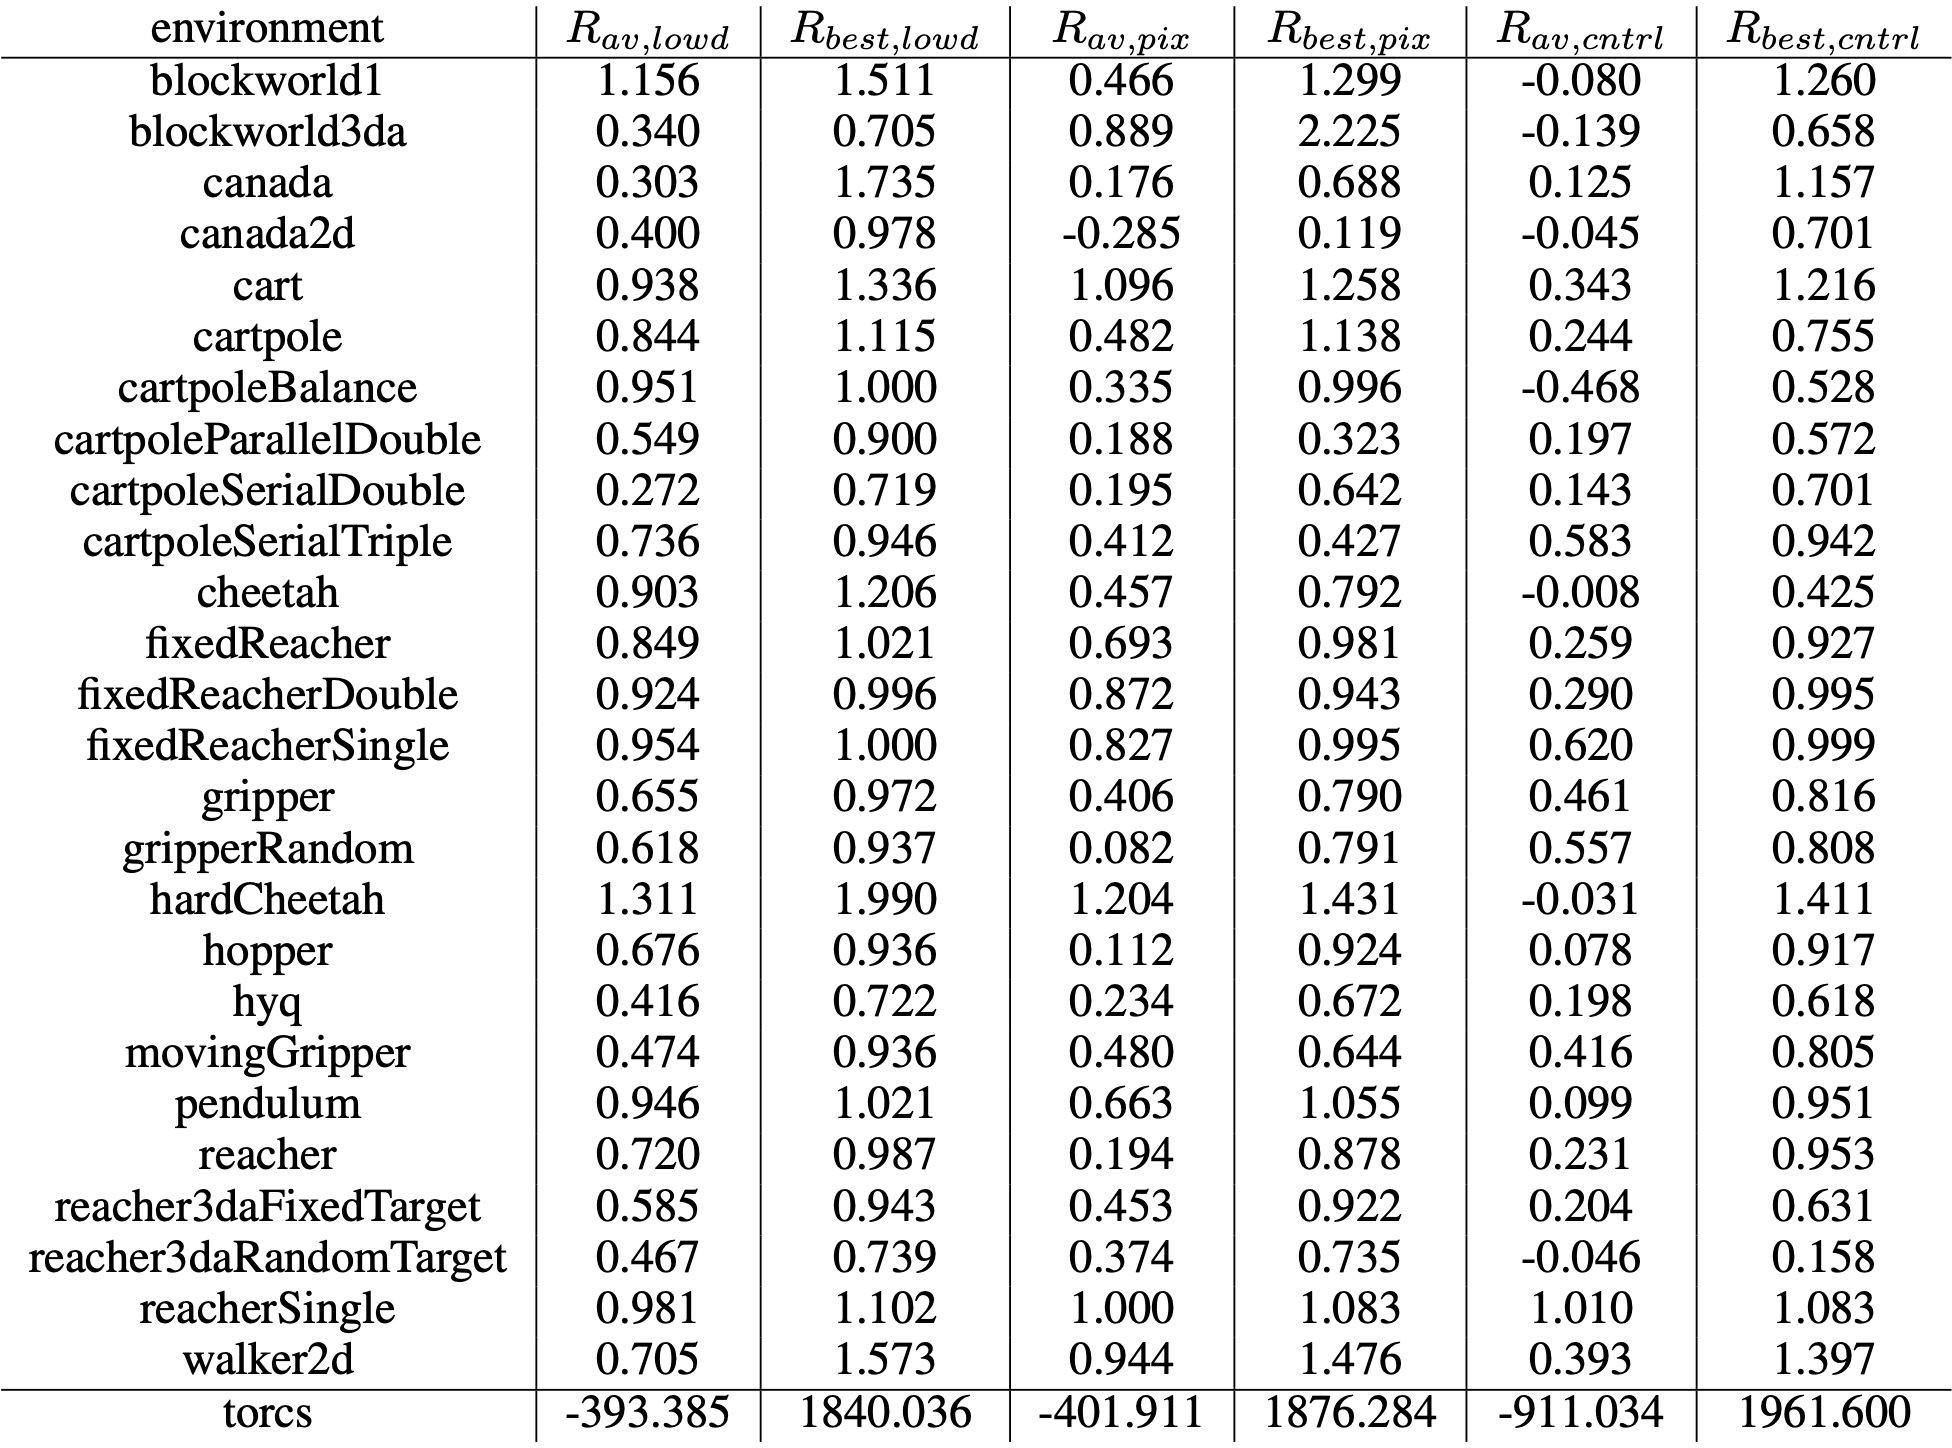
\includegraphics[width=\linewidth,height=0.78\textheight,keepaspectratio]{images/ddpg/figures/ddpg-vs-dpg-table.jpg}};
\begin{scope}[shift={(tbl.south west)}, x={($(tbl.south east)-(tbl.south west)$)}, y={($(tbl.north west)-(tbl.south west)$)}]
  \ddpgdpglabels
\end{scope}
\end{tikzpicture}
\end{column}
\end{columns}
\end{frame}

% Slide 54: + tall red box around DDPG "lowd" pair (R_av,lowd + R_best,lowd)
\begin{frame}{Experiments}
\begin{columns}[c]
\begin{column}{0.22\textwidth}
\centering
\large\textbf{Is DDPG better than DPG?}
\end{column}
\begin{column}{0.78\textwidth}
\begin{tikzpicture}
\node[inner sep=0] (tbl) {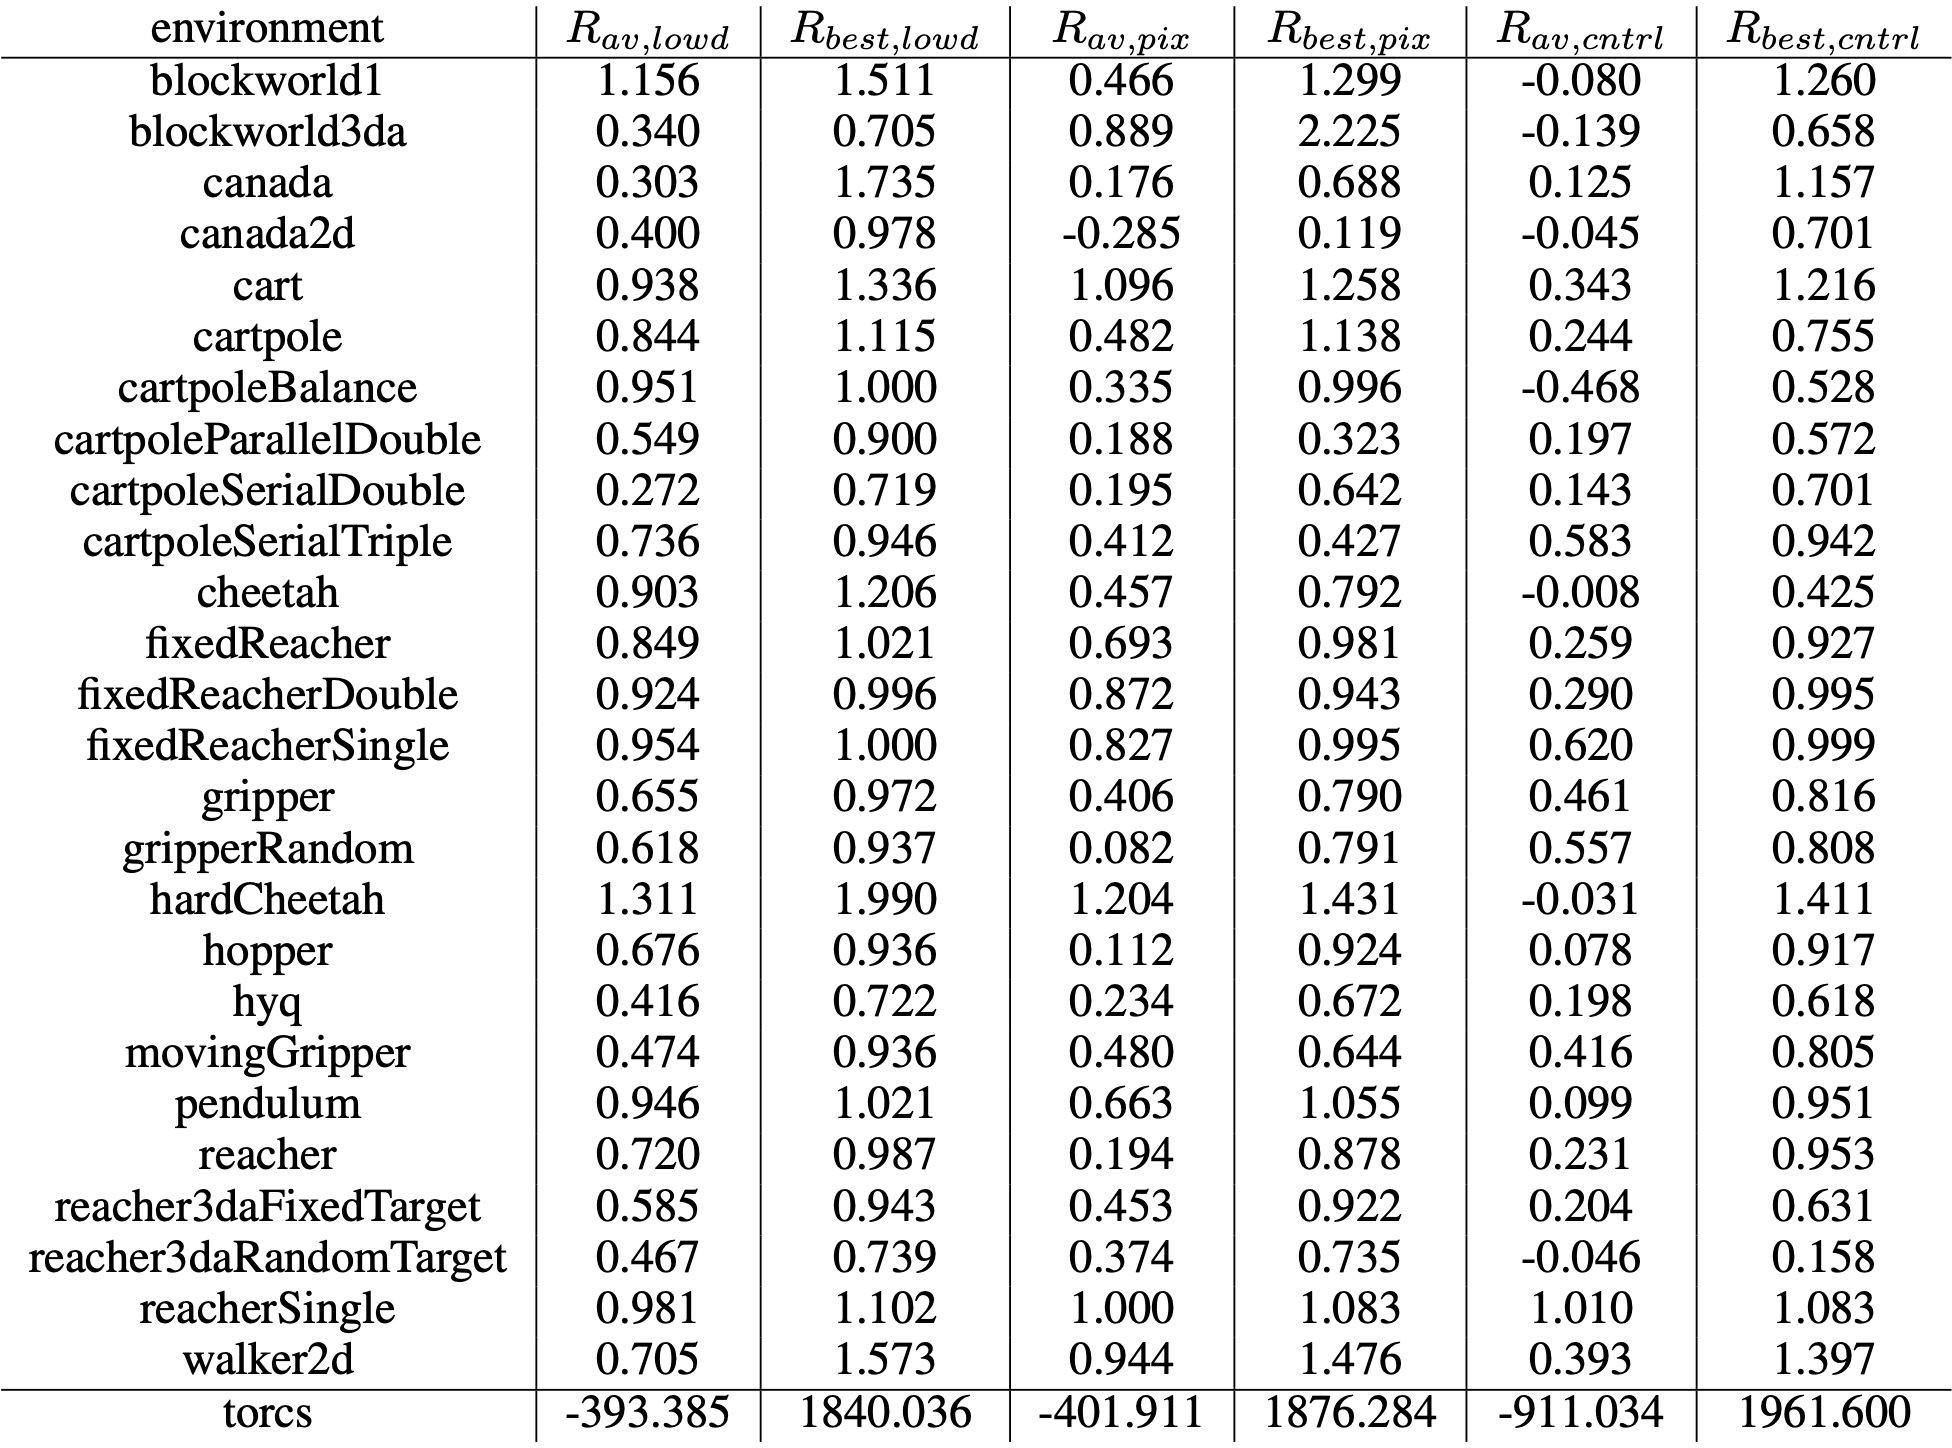
\includegraphics[width=\linewidth,height=0.78\textheight,keepaspectratio]{images/ddpg/figures/ddpg-vs-dpg-table.jpg}};
\begin{scope}[shift={(tbl.south west)}, x={($(tbl.south east)-(tbl.south west)$)}, y={($(tbl.north west)-(tbl.south west)$)}]
  \ddpgdpglabels
  \draw[red,line width=0.8pt] (0.225, 0.04) rectangle (0.45, 0.945);
\end{scope}
\end{tikzpicture}
\end{column}
\end{columns}
\end{frame}

% Slide 55: + tall red box around DDPG "pix" pair (R_av,pix + R_best,pix)
\begin{frame}{Experiments}
\begin{columns}[c]
\begin{column}{0.22\textwidth}
\centering
\large\textbf{Is DDPG better than DPG?}
\end{column}
\begin{column}{0.78\textwidth}
\begin{tikzpicture}
\node[inner sep=0] (tbl) {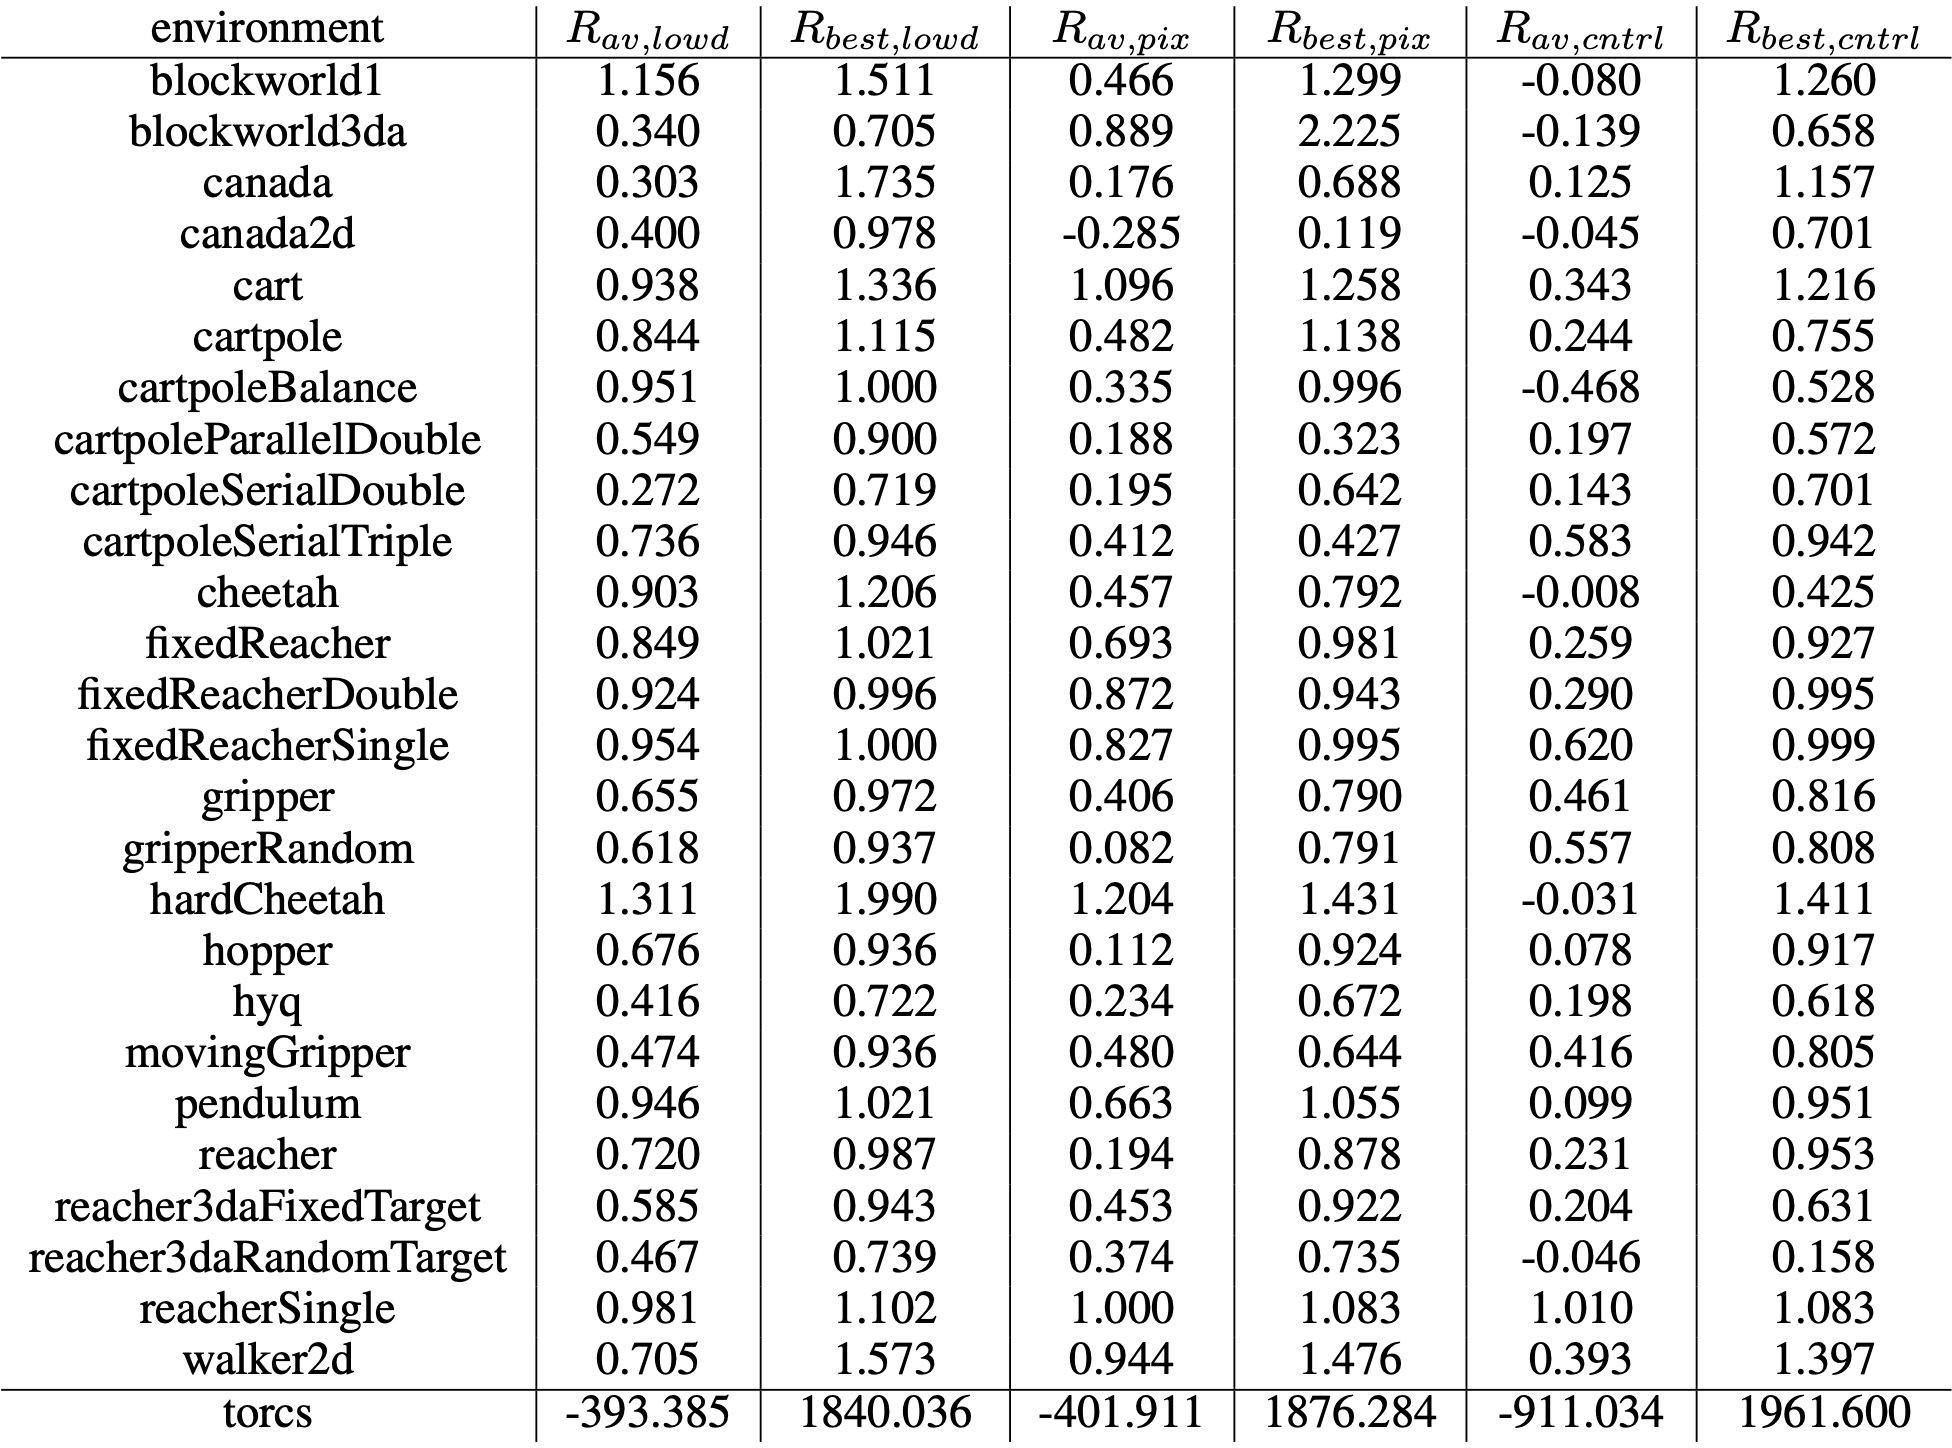
\includegraphics[width=\linewidth,height=0.78\textheight,keepaspectratio]{images/ddpg/figures/ddpg-vs-dpg-table.jpg}};
\begin{scope}[shift={(tbl.south west)}, x={($(tbl.south east)-(tbl.south west)$)}, y={($(tbl.north west)-(tbl.south west)$)}]
  \ddpgdpglabels
  \draw[red,line width=0.8pt] (0.45, 0.04) rectangle (0.66, 0.945);
\end{scope}
\end{tikzpicture}
\end{column}
\end{columns}
\end{frame}

% Slide 56: + tall red box around DPG "cntrl" pair (R_av,cntrl + R_best,cntrl)
\begin{frame}{Experiments}
\begin{columns}[c]
\begin{column}{0.22\textwidth}
\centering
\large\textbf{Is DDPG better than DPG?}
\end{column}
\begin{column}{0.78\textwidth}
\begin{tikzpicture}
\node[inner sep=0] (tbl) {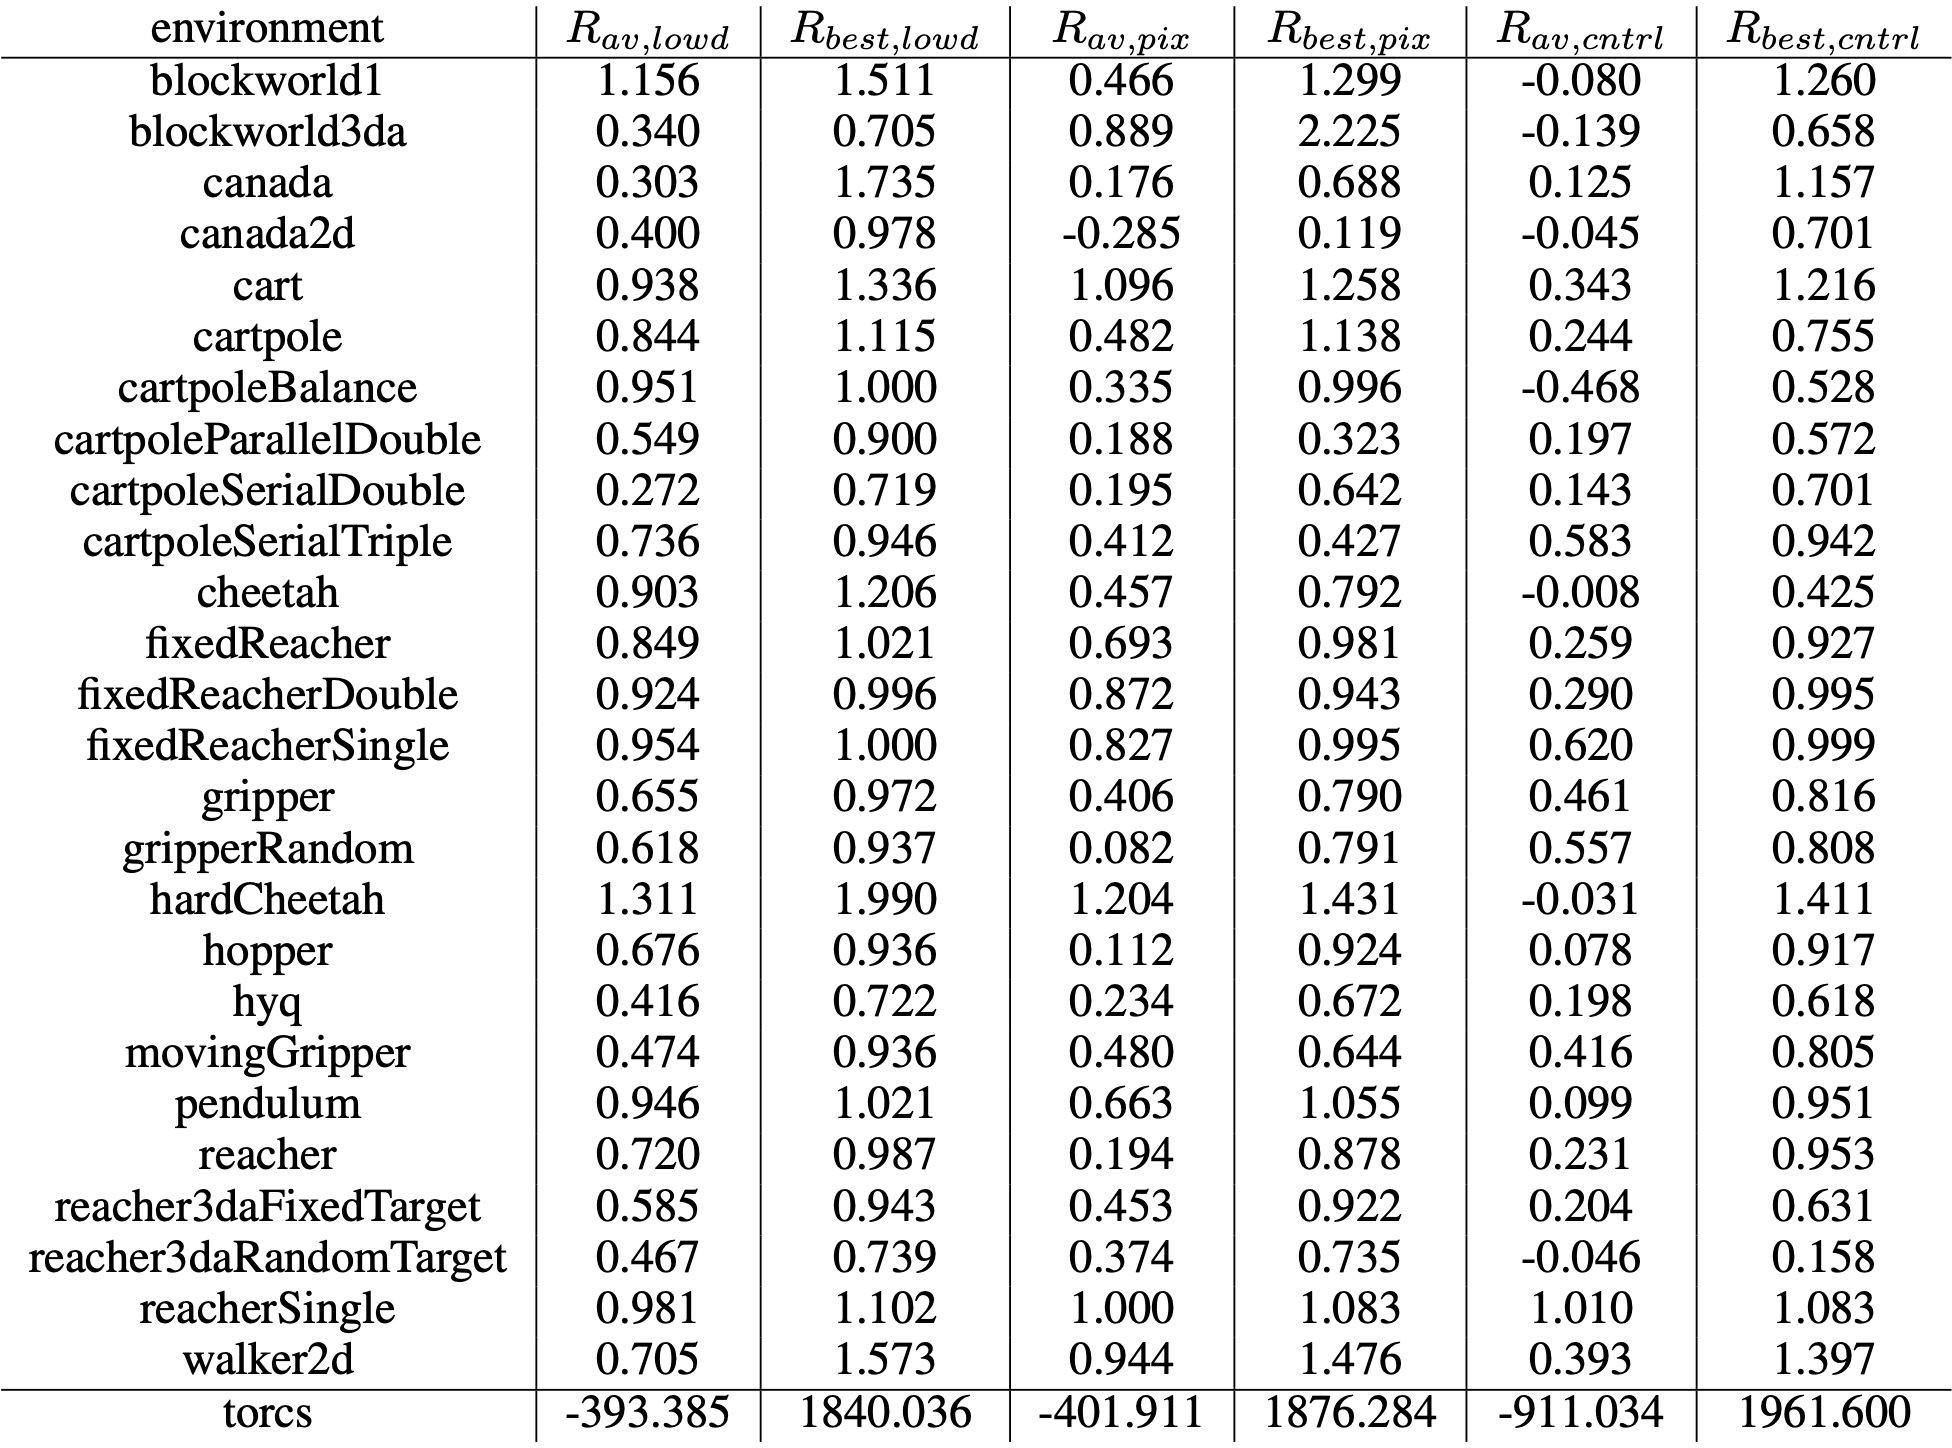
\includegraphics[width=\linewidth,height=0.78\textheight,keepaspectratio]{images/ddpg/figures/ddpg-vs-dpg-table.jpg}};
\begin{scope}[shift={(tbl.south west)}, x={($(tbl.south east)-(tbl.south west)$)}, y={($(tbl.north west)-(tbl.south west)$)}]
  \ddpgdpglabels
  \draw[red,line width=0.8pt] (0.74, 0.04) rectangle (0.985, 0.945);
\end{scope}
\end{tikzpicture}
\end{column}
\end{columns}
\end{frame}

% Slide 57: red box back at DDPG lowd pair + "DDPG still exhibits high variance" callout
\begin{frame}{Experiments}
\begin{columns}[c]
\begin{column}{0.22\textwidth}
\centering
\textcolor{red}{\textbf{DDPG still exhibits high variance}}
\end{column}
\begin{column}{0.78\textwidth}
\begin{tikzpicture}
\node[inner sep=0] (tbl) {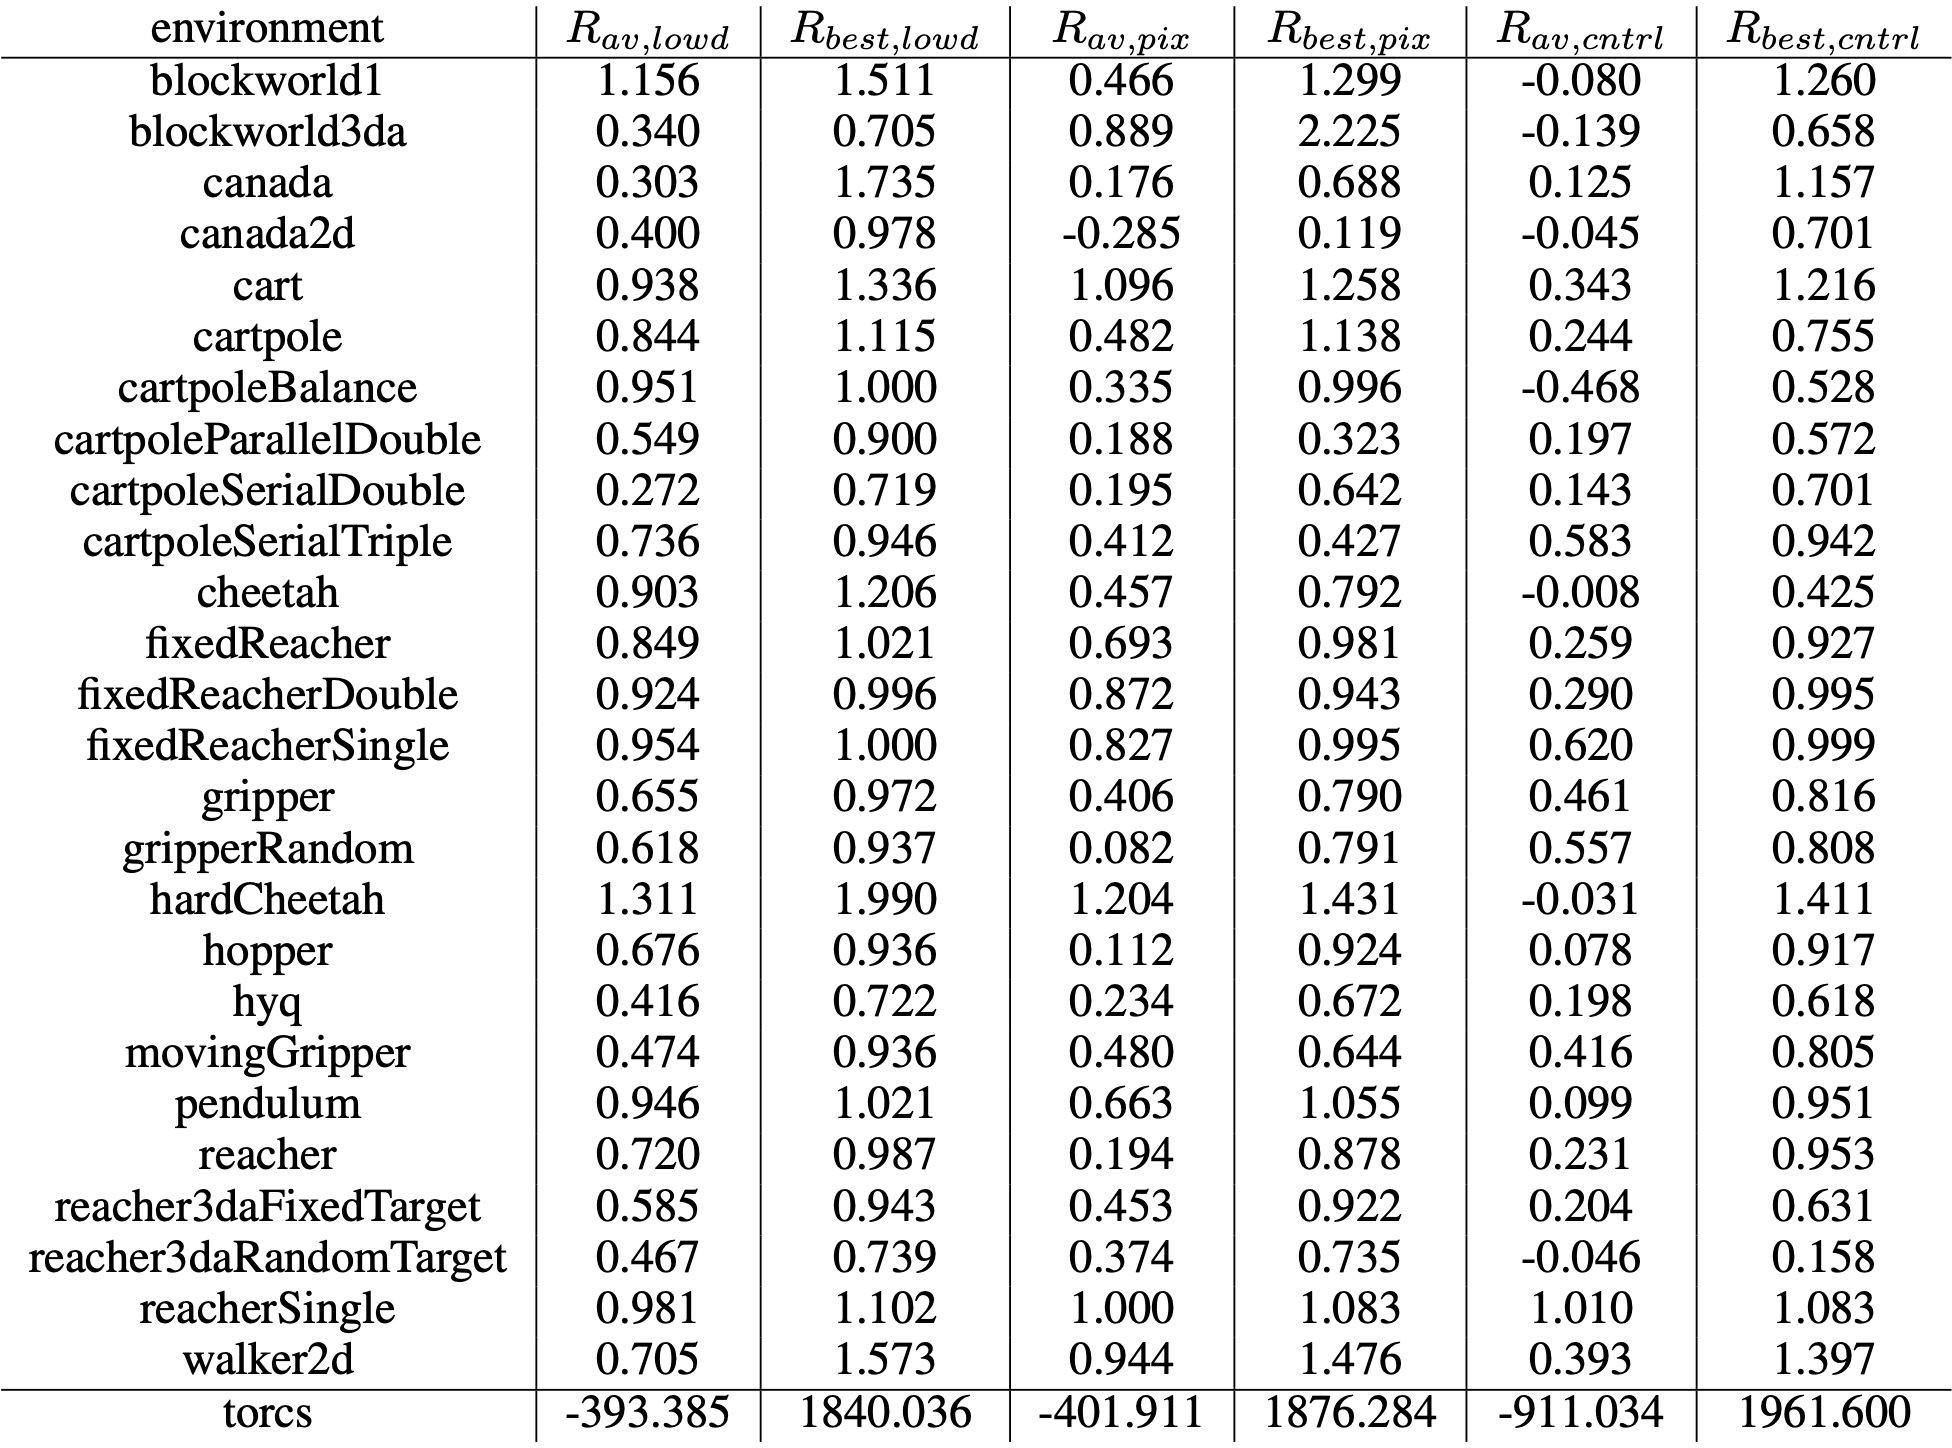
\includegraphics[width=\linewidth,height=0.78\textheight,keepaspectratio]{images/ddpg/figures/ddpg-vs-dpg-table.jpg}};
\begin{scope}[shift={(tbl.south west)}, x={($(tbl.south east)-(tbl.south west)$)}, y={($(tbl.north west)-(tbl.south west)$)}]
  \ddpgdpglabels
  \draw[red,line width=0.8pt] (0.225, 0.04) rectangle (0.45, 0.945);
\end{scope}
\end{tikzpicture}
\end{column}
\end{columns}
\end{frame}
